\section{Evaluering og diagnostisering}

Hvor god en modell er avhenger av hvilket formål modellen skal brukes til. Skal
modellen brukes til å komme med en punktprediksjon kan det være at man ønsker
at modellen skal ha lav absolutt feil. I andre tilfeller er man interessert i at
modellen skal gjenspeile spredningen i observasjonene. Vel så viktig kan det
være å estimere sannsynligheten for at det kommer en eller flere hendelser i
neste uke, $P(Y_{i, t+1} > 0)$, som det er å prøve å estimere den faktiske
størrelsen. For å komme med estimater på sannsynligheter for intervaller av
verdier er det nødvendig at den prediktive fordelingen passer til de observerte
dataene. Hvor godt modellen beskriver dataene kalles kalibrering. Hvor godt
modellen er kalibrert kan bedømmes gjennom diagnostiske plot. Hvor konsentrert
modellen er rundt punktestimatet kalles for skarphet. Skarphet kan bedømmes
gjennom \textit{scoring rules} \parencite{czado2009predictive}. 


\subsection{Kvadrert feil}

For å se på hvor godt modellene gjør punktprediksjoner er den kvadrerte feilen
(RMSE) av interesse.  Det er viktig å være oppmerksom på at prediksjonene her
gjøres på de samme dataene som er brukt til å estimere parametrene i modellene,
og man kan få overtilpassede modeller hvis man bare ser på RMSE.  

$$
\mathrm{RMSE}=\sqrt{\frac{1}{n}\sum_{i=1}^n(\hat{y}_i-y_i)^2}
$$

RMSE sier imidlertid ingenting om variansen. For å se på feilen relativ til
hvor stor spredning modellen estimerer kan man normalisere feilen ved å dele på
variansen (RMNSE). Også ved bruk RMNSE som et mål på hvor godt modellene gjør
må man være varsom. En modell som overestimerer variansen vil ha lavere RMNSE
sammenlignet med en modell med samme forventning, men lavere varians.

$$
\mathrm{RMNSE}=\sqrt{\frac{1}{n}\sum_{i=1}^n \left(\frac{\hat{y}_i-y_i}{\hat{\sigma}_i}\right)^2}
$$

\subsection{Scoring rules}

En scoring rule er en oppsummering av modellen og observasjonene i form av et
tall. Når man sammenligner modeller svarer et lavere tall til en modell som
beskriver dataene bedre. Fra \citep{czado2009predictive} er en scoring rule er
proper hvis for en fordeling $Q$ en fordeling $P$ og en scoring rule $s$ har
følgende forhold:

\begin{equation}
s(Q, Q) \leq s(P, Q)
    \label{eq:proper}
\end{equation}

Her er $Q$ fordelingen som etter modellererens dømme er den sanne fordelingen
av dataene. Hvis (\ref{eq:proper}) har likhet kun hvis $P = Q$ er $s$ strikt
proper. Strikt propre scoring rules gir et mål på både kalibrering og skarphet. 

En proper scoring rule er Dawid-Sebastini score
\parencite{gneiting2007strictly}. Den inkorporerer variansen og standardisert
feil samtidig. 


$$
\mathrm{DS}(P, x) =\frac{1}{n}\sum_{i=1}^n \left(\frac{\hat{y}_i - y_i}{\hat{\sigma}_i}\right)^2 + 2 \log \hat{\sigma}_i.
$$

I DS-scoren øker det andre leddet når variansen øker. Motsatt øker det første
leddet hvis variansen synker. En annen scoring rule som både tar hensyn til
punkt-prediksjonen og prediksjonsintervallet er \textit{Ranked Probability
Score (RPS)}. RPS til en observasjon $x$ kan skrives som 

$$
RPS(P_i,x) = \frac{1}{n}\sum_{i=1}^n \mathrm{E}|X - y_i| - \frac{1}{2}\mathrm{E}|X - X'|,
$$

\noindent
der $P_i$ er en betinget sannsynlighetsfordeling. $X$ og $X'$ er to uavhengige
variabler fra fordelingen $P_i$ \parencite{gneiting2007strictly}. Har $P_i$
stor spredning vil både første og andre ledd øke. Samtidig vil en $P_i$ som
legger mye vekt rundt $y_i$ gi lave verdier i det første leddet.

\subsection{PIT-diagram}

En annen måte å diagnostisere modellene på er å plotte de predikerte kvantilene
i den observerte fordelingen mot kvantilene i den prediktive fordelingen. I
\citep{czado2009predictive} anbefales det å plotte et Probability Integral
Transform (PIT) diagram for å undersøke om den prediktive distribusjonen
beskriver de observerte dataene. For diskrete data foreslår
\citep{czado2009predictive} følgende måte å regne ut PIT-score for et utvalg.
For en verdi $u \in [0, 1]$ og en observasjon $y$ regner man først ut 

$$
F(u|y) = \begin{cases}
    0, & \quad u < P_{y-1} \\
    \frac{u - P_{y-1}}{P_y - P_{y-1}}, & \quad P_{y-1} \leq u \leq P_y \\
    1, & \quad P_y < u
         \end{cases}  
.
$$

Her er $P$ den kumulative tetthetsfunksjonen for $y_t | y_{t-1}$. For å
diagnostiserer modellen kan man se på $\overline{F}(u) =
\frac{1}{n}\sum_{i=1}^nF(u|y_i)$. Hvis $y \sim P$ så vil $\overline{F}(u)$ gå
mot $u$ når $n \to \infty$. Nå kan man plotte $\overline{F}(u)$ mot $u$, eller
så kan man definere en ny variabel:

$$
F(j)= \overline{F}\left(\frac{j}{J}\right) 
- \overline{F}\left(\frac{j-1}{J}\right),
$$

\
der $j \in \{1\,2,\ldots,J \}$ for en valgt verdi av $J$. Lager man et
histogram der søylene har høyde $F(j)$ vil strukturen på histogrammet gi
informasjon om hvordan de observerte verdiene forholder seg til
prediksjonsfordelingen. Hvis observasjonene $y \sim P$ vil søylene være nær
like høye for alle $j$. Et histogram med form som en u snudd opp ned indikerer
at den observerte fordelingen er tettere enn det som er forventet under den
estimerte fordelingen. Motsatt vil et u-formet histogram indikere at modellen
forventer lavere spredning en det som er observert. I \cref{fig:pit_explain}
ser man et eksempel med simulerte data. PIT-histogrammer for 200 verdier
trukket fra en negativ binomialfordeling med parametere $r=5$ og $p=0.5$. 

    \begin{figure}[!h]
    \centering
    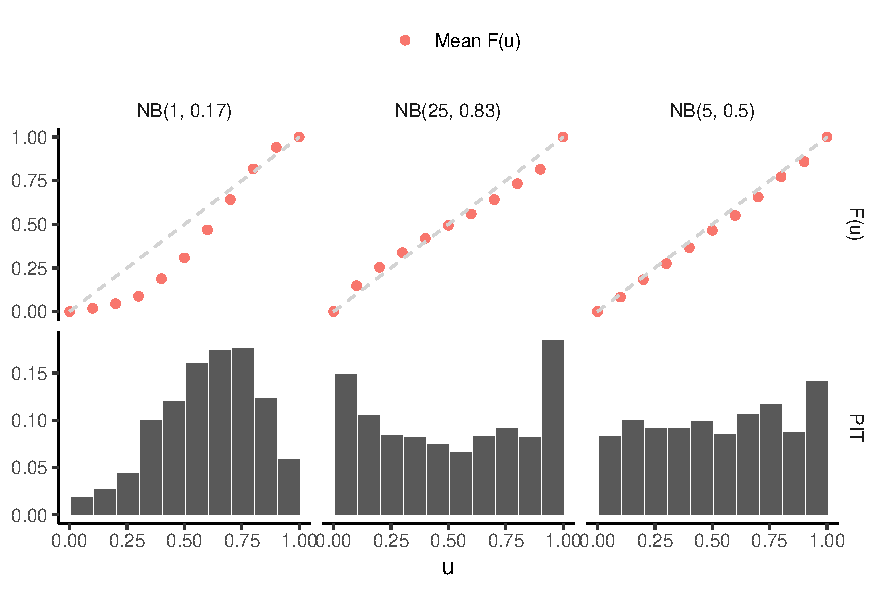
\includegraphics{../img/pit_explain.pdf}
    \caption{
        $F(u)$ og PIT-diagram for 200 tilfeldige verdier trukket fra en
        $\mathrm{NB}(5, 0.5)$-fordeling, med forventning 5 og varians 10.
        $F(u)$ og PIT-diagrammet er regnet ut fra 3 fordelinger med forventning
        5, men med forskjellig varians. I den første raden ses
        $\overline{F}(u)$, den nederste raden viser PIT-diagrammet. I den
        første kolonnen er en modell med overspredning (varians 150). Den andre
        kolonnen viser $F(u)$ og PIT-diagram for en modell med underspredning
        (varians $\frac{6}{5}$) Den siste kolonnen viser $F(u)$ og PIT-diagram
        regnet ut fra originalfordelingen. Eksemplet er adaptert fra
        \cite{czado2009predictive}
    }
        \label{fig:pit_explain}
    \end{figure}

